% Comment lines start with %
% LaTeX commands start with \
% This template was provided by Jennifer Welch for CSCE 222-200, Honors, Spring 2015

\documentclass[12pt]{article}  % This is an article with font size 12-point

% Packages add features
\usepackage{times}     % font choice
\usepackage{amsmath}   % American Mathematical Association math formatting
\usepackage{amsthm}    % nice formatting of theorems
\usepackage{amssymb}    % provides some symbols
\usepackage{latexsym}  % provides some more symbols
\usepackage{fullpage}  % uses most of the page (1-inch margins)
\usepackage[shortlabels]{enumitem}
\usepackage{graphicx}
\usepackage{tikz}

\setlength{\parskip}{.1in}  % increase the space between paragraphs

\renewcommand{\baselinestretch}{1.1}  % increase the space between lines

% Convenient renaming of symbols for logic formulas
\newcommand{\NOT}{\neg}
\newcommand{\AND}{\wedge}
\newcommand{\OR}{\vee}
\newcommand{\XOR}{\oplus}
\newcommand{\IMPLIES}{\rightarrow}
\newcommand{\IFF}{\leftrightarrow}
\providecommand{\myceil}[1]{$\left \lceil #1 \right \rceil$}
\providecommand{\myfloor}[1]{$\left \lfloor #1 \right \rfloor$}
\newcommand{\powerset}[1]{\mathbb{P}(#1)}

% Actual content starts here.
\begin{document}

\begin{center}         % center all the material between begin and end
{\large                % use larger font
CSCE 222 (Carlisle), Discrete Structures for Computing \\  % \\ is line break
Spring 2022 \\
Homework 13}
\end{center}
\rule{6in}{.1pt}       % horizontal line 6 inches long and .1 point high
\begin{center}
{\large
Type your name below the pledge to sign\\
On my honor, as an Aggie, I have neither given nor received unauthorized aid on this academic work.\\
Huy QUANG LAI}
\end{center}

% blank line separates paragraphs.  First line of a paragraph is automatically
% indented.  

\rule{6in}{.1pt}       % horizontal line 6 inches long and .1 point high
                    
\noindent              % don't indent
{\bf Instructions:}    % \bf makes text boldface
                       % \em makes text emphasized (italics)

\begin{itemize}        % makes an itemized list
\item The exercises are from the textbook.  You are encouraged to work
      extra problems to aid in your learning; remember, the solutions to 
      the odd-numbered problems are in the back of the book.
\item Grading will be based on correctness, clarity, and whether your
      solution is of the appropriate length.
\item Always justify your answers.
\item Don't forget to acknowledge all sources of assistance in the section below, and write up your solutions on your own.
\item {\em Turn in .pdf file to Gradescope by the start of class on Monday, May 2, 2022.}  It is simpler to put each problem on its own page using the LaTeX clearpage command.
\end{itemize}


\rule{6in}{.1pt}       % horizontal line 6 inches long and .1 point high

{\bf Help Received:}    % \bf makes text boldface
\begin{itemize}
\item Rosen, Kenneth H. \textit{Discrete Mathematics and Its Applications}. McGraw-Hill, 2019.
\item Wallace, Evan. \textit{Finite State Machine Designer}, 2010, madebyevan.com/fsm/. 
\end{itemize}



\rule{6in}{.1pt}       % horizontal line 6 inches long and .1 point high

%---------------------------------------------------------------------

% \subsection makes a subsection heading; * leaves it unnumbered.
% (Usually subsections are inside sections, but the \section command
% used a font that was larger than I wanted.)
\subsection*{Exercises for Section 13.1:}     

\noindent
{\bf 4(a-c): (3 points).}

\noindent
Let $G=(V,T,S,P)$ be the phrase-structure grammar with $V=\{0, 1, A, S\},T=\{0, 1\}$, and set of productions $P$ consisting of $S\to1S,S\to00A,A\to0A$, and $A\to0.$
\begin{enumerate}[a)]
    \item Show that 111000 belongs to the language generated by $G$.\\
    $S\Rightarrow1S\Rightarrow11S\Rightarrow111S\Rightarrow11100A\Rightarrow111000$
    \item Show that 11001 does not belong to the language generated by $G$.\\
    Every production results in a string ending in $S,A$ or $0$. Therefore, any string ending with $1$ is not possible.
    \item What is the language generated by $G$?\\
    The string can start any number of 1’s, including zero, by iterating the production $S\to1S$.\\
    Eventually the $S$ must turn into $00A$, so at least two 0’s must come next.\\
    The string can then contain additional 0's using $A\to0A$ repeatedly.\\
    Because $A\to0$ is called at the end, this adds at least one more 0 (and therefore a total of at least three 0’s).\\
    So the language generated by $G$ is the set of all strings consisting of zero or more 1’s followed by three or more 0’s. We can write this as $\{0^n1^m\vert n\geq0$ and $m\geq3 \}$.
    
\end{enumerate}

\noindent
{\bf 18(a,c): (2 points).}

\noindent
Construct phrase-structure grammars to generate each of these sets.
\begin{enumerate}[a)]
    \item $\{01^{2n}\vert n\geq0\}$\\
    Exactly one 0. Followed by an even number of 1.\\
    $S\to0A$\\
    $A\to11A$\\
    $A\to\lambda$
    
    \setcounter{enumi}{2}
    \item $\{0^n1^m0^n\vert m\geq0\textrm{ and }n\geq0\}$\\
    Grow 0's from the center. Convert the center into a 1-making machine.\\
    $S\to0S0$\\
    $S\to A$\\
    $A\to1A$\\
    $A\to\lambda$
\end{enumerate}

\clearpage
\noindent
{\bf 24b: (1 point).}

\noindent
Let $G$ be the grammar with $V=\{a,b,c,S\};T=\{a, b, c\}$; starting symbol $S$; and productions $S\to abS, S\to bcS,S\to bbS,S\to a,$ and $S\to cb$. Construct derivation trees for $bbbcbba$.
\begin{enumerate}
    \item $S\to bbS$
    \item $S\to bcS$
    \item $S\to bbS$
    \item $S\to a$
\end{enumerate}

\clearpage
\subsection*{Exercises for Section 13.2:}     

\noindent
{\bf 4(a-c): (3 points).}

\noindent
Find the output generated from the input string $10001$ for the finite-state machine with the state diagram in
\begin{enumerate}[a)]
    \item Exercise 2(a).\\
    The machine starts in state $s_0$.\\
    On input $1$, it moves to state $s_2$ and outputs $0$.\\
    The next three inputs of 0's drive it to state $s_3$, then to $s_1$, then back to $s_0$. This will output $011$.\\
    The final $1$ drives it back to $s_2$ and outputs $0$.\\
    The output is $00110$.
    \item Exercise 2(b).\\
    The machine starts in state $s_0$.\\
    On input $1$, it moves to state $s_2$ and outputs $1$.\\
    The next three inputs of 0's keep it at $s_2$, outputting $1$ each time.
    The final $1$ drives it back to $s_0$ and outputs $0$.\\
    The output is $11110$.
    \item Exercise 2(c).\\
    The machine starts in state $s_0$.\\
    On input $1$, it moves to state $s_1$ and gives $1$ as output.\\
    The next input symbol is $0$, so the machine moves back to state $s_0$ and gives $0$ as output.\\
    The third input is $0$, so the machine moves to state $s_3$ and gives $0$ as output.\\
    The fourth input is $0$, so the machine moves to state $s_1$ and gives $0$ as output.\\
    The fifth input is $1$, so the machine stays in state $s_1$ and gives $1$ as output.\\
    The output is $10001$.
\end{enumerate}

\clearpage
\noindent
{\bf 16: (2 points).}

\noindent
Construct a finite-state machine that gives an output of $1$ if the number of input symbols read so far is divisible by $3$ and an output of $0$ otherwise.
\begin{center}
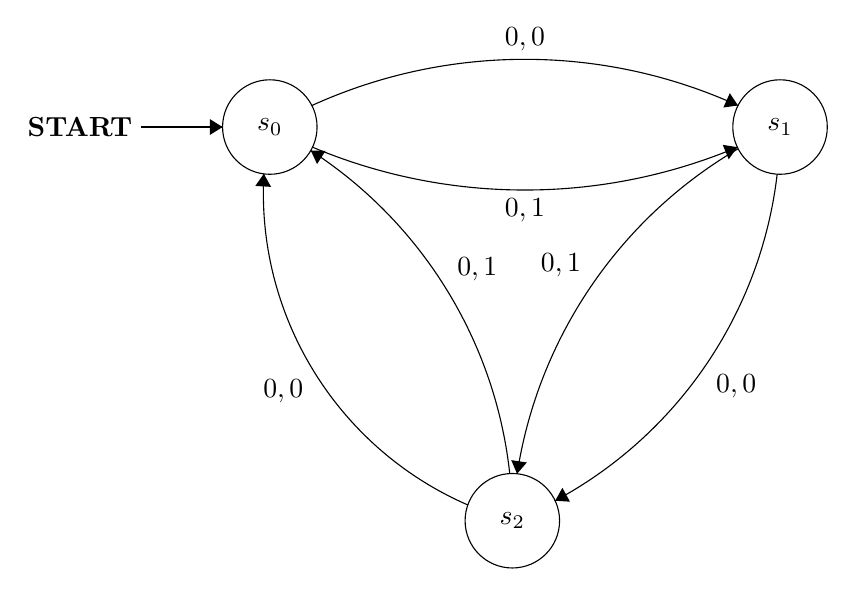
\begin{tikzpicture}[scale=0.2]
\tikzstyle{every node}+=[inner sep=0pt]
\draw [black] (20.9,-17.9) circle (3);
\draw (20.9,-17.9) node {$s_0$};
\draw [black] (53.3,-17.9) circle (3);
\draw (53.3,-17.9) node {$s_1$};
\draw [black] (36.3,-42.9) circle (3);
\draw (36.3,-42.9) node {$s_2$};
\draw [black] (23.57,-16.534) arc (114.47503:65.52497:32.659);
\fill [black] (50.63,-16.53) -- (50.11,-15.75) -- (49.7,-16.66);
\draw (37.1,-13.1) node [above] {$0,0$};
\draw [black] (50.588,-19.18) arc (-67.19709:-112.80291:34.802);
\fill [black] (50.59,-19.18) -- (49.66,-19.03) -- (50.04,-19.95);
\draw (37.1,-22.4) node [below] {$0,1$};
\draw [black] (53.117,-20.893) arc (-6.67228:-61.75912:27.115);
\fill [black] (39.02,-41.63) -- (39.96,-41.69) -- (39.48,-40.81);
\draw (49.21,-34.34) node [right] {$0,0$};
\draw [black] (36.605,-39.917) arc (171.20578:120.36281:29.067);
\fill [black] (36.6,-39.92) -- (37.22,-39.2) -- (36.23,-39.05);
\draw (40.69,-26.67) node [left] {$0,1$};
\draw [black] (33.475,-41.898) arc (-113.49768:-183.23619:21.596);
\fill [black] (20.52,-20.87) -- (19.98,-21.64) -- (20.98,-21.7);
\draw (23.06,-34.7) node [left] {$0,0$};
\draw [black] (23.5,-19.394) arc (57.05556:6.21058:28.06);
\fill [black] (23.5,-19.39) -- (23.9,-20.25) -- (24.44,-19.41);
\draw (32.77,-26.94) node [right] {$0,1$};
\draw [black] (12.7,-17.9) -- (17.9,-17.9);
\draw (12.2,-17.9) node [left] {\textbf{START}};
\fill [black] (17.9,-17.9) -- (17.1,-17.4) -- (17.1,-18.4);
\end{tikzpicture}
\end{center}

\clearpage
\subsection*{Exercises for Section 13.3:}     

\noindent
{\bf 10(a,c,e): (3 points).}

\noindent
Determine whether the string $01001$ is in each of these sets
\begin{enumerate}[a)]
    \item \{0,1\}*\\
    This is the set of all bit strings. Therefore, the string is within the set.
    
    \setcounter{enumi}{2}
    \item \{010\}*\{0\}*\{1\}\\
    The string is $(010)^10^11$ so it is in the set.
    
    \setcounter{enumi}{4}
    \item \{00\}\{0\}*\{01\}\\
    Any string in this set must start with 00. Since the string does not, the string is not in the set.
\end{enumerate}

\noindent
{\bf CUSTOM: Create a DFA that recognizes binary numbers that are a multiple of 3: (2 points).}

\begin{center}
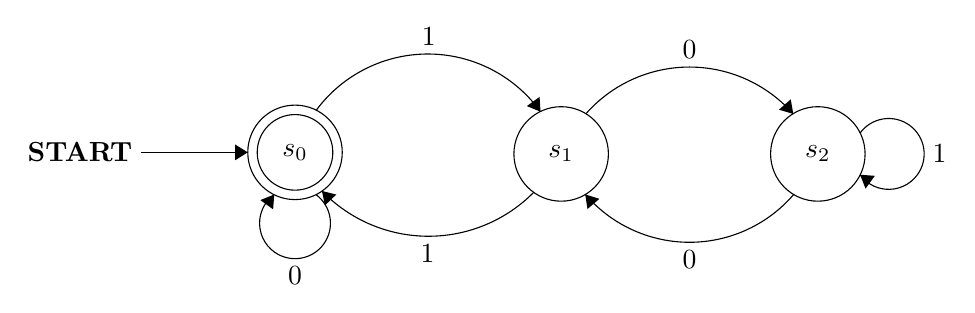
\begin{tikzpicture}[scale=0.2]
\tikzstyle{every node}+=[inner sep=0pt]
\draw [black] (26.4,-15.5) circle (3);
\draw [black] (26.4,-15.5) circle (2.4);
\draw (26.4,-15.5) node {$s_0$};
\draw [black] (43.3,-15.6) circle (3);
\draw (43.3,-15.6) node {$s_1$};
\draw [black] (59.6,-15.6) circle (3);
\draw (59.6,-15.6) node {$s_2$};
\draw [black] (16.6,-15.5) -- (23.4,-15.5);
\draw (16.1,-15.5) node [left] {\textbf{START}};
\fill [black] (23.4,-15.5) -- (22.6,-15) -- (22.6,-16);
\draw [black] (27.723,-18.18) arc (54:-234:2.25);
\draw (26.4,-22.75) node [below] {$0$};
\fill [black] (25.08,-18.18) -- (24.2,-18.53) -- (25.01,-19.12);
\draw [black] (27.742,-12.833) arc (143.5405:35.78145:8.819);
\fill [black] (41.99,-12.92) -- (41.93,-11.98) -- (41.12,-12.56);
\draw (34.89,-8.75) node [above] {$1$};
\draw [black] (44.864,-13.057) arc (138.61182:41.38818:8.778);
\fill [black] (58.04,-13.06) -- (57.88,-12.13) -- (57.13,-12.79);
\draw (51.45,-9.58) node [above] {$0$};
\draw [black] (58.074,-18.165) arc (-40.60451:-139.39549:8.724);
\fill [black] (44.83,-18.17) -- (44.97,-19.1) -- (45.73,-18.45);
\draw (51.45,-21.71) node [below] {$0$};
\draw [black] (62.28,-14.277) arc (144:-144:2.25);
\draw (66.85,-15.6) node [right] {$1$};
\fill [black] (62.28,-16.92) -- (62.63,-17.8) -- (63.22,-16.99);
\draw [black] (41.565,-18.032) arc (-44.65343:-136.02461:9.405);
\fill [black] (28.11,-17.95) -- (28.3,-18.87) -- (29.02,-18.18);
\draw (34.82,-21.33) node [below] {$1$};
\end{tikzpicture}
\end{center}

\noindent
{\bf 20: (2 points).}
\begin{center}
    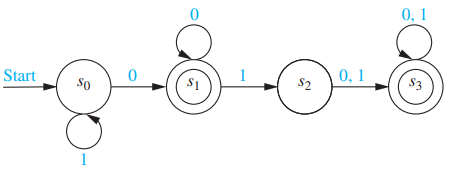
\includegraphics[]{images/HW13q20.PNG}
\end{center}

\noindent
\{$1$\}*\{$0$\}\{$0$\}*$\bigcup$\{$1$\}*\{$0$\}\{$0$\}*\{$10,11$\}\{$0,1$\}*

\clearpage
\noindent
{\bf 26: (2 points).}

\noindent
Construct a deterministic finite-state automaton that recognizes the set of all bit strings that do not contain three consecutive 0s.

\noindent
Have four states, with only $s_3$ non-final. For $i=0,1,2$, transition from $s_i$ to $s_{i+1}$ on input $0$ but back to $s_0$ on input $1$. Both transitions from $s_3$ are to itself.

\begin{center}
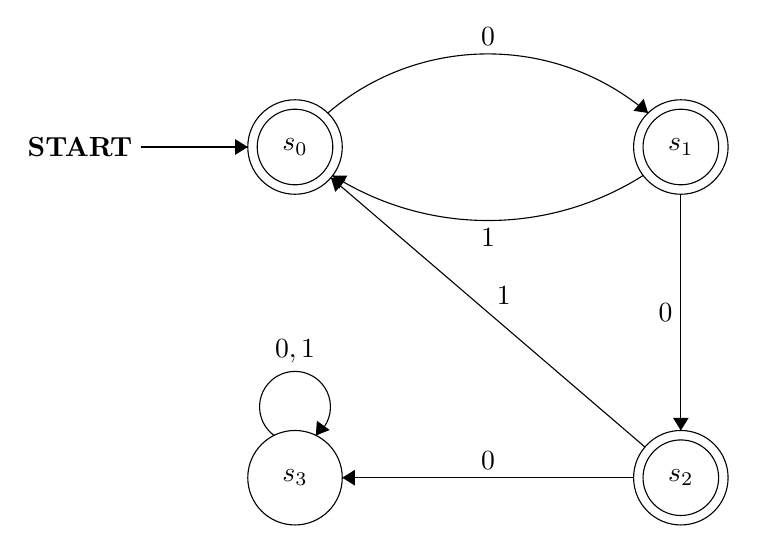
\begin{tikzpicture}[scale=0.2]
\tikzstyle{every node}+=[inner sep=0pt]
\draw [black] (24.8,-13.1) circle (3);
\draw (24.8,-13.1) node {$s_0$};
\draw [black] (24.8,-13.1) circle (2.4);
\draw [black] (49.3,-13.1) circle (3);
\draw (49.3,-13.1) node {$s_1$};
\draw [black] (49.3,-13.1) circle (2.4);
\draw [black] (49.3,-34.1) circle (3);
\draw (49.3,-34.1) node {$s_2$};
\draw [black] (49.3,-34.1) circle (2.4);
\draw [black] (24.8,-34.1) circle (3);
\draw (24.8,-34.1) node {$s_3$};
\draw [black] (26.879,-10.944) arc (130.54606:49.45394:15.646);
\fill [black] (47.22,-10.94) -- (46.94,-10.04) -- (46.29,-10.8);
\draw (37.05,-6.69) node [above] {$0$};
\draw [black] (46.909,-14.906) arc (-57.61215:-122.38785:18.405);
\fill [black] (27.19,-14.91) -- (27.6,-15.76) -- (28.13,-14.91);
\draw (37.05,-18.27) node [below] {$1$};
\draw [black] (49.3,-16.1) -- (49.3,-31.1);
\fill [black] (49.3,-31.1) -- (49.8,-30.3) -- (48.8,-30.3);
\draw (48.8,-23.6) node [left] {$0$};
\draw [black] (46.3,-34.1) -- (27.8,-34.1);
\fill [black] (27.8,-34.1) -- (28.6,-34.6) -- (28.6,-33.6);
\draw (37.05,-33.6) node [above] {$0$};
\draw [black] (47.02,-32.15) -- (27.08,-15.05);
\fill [black] (27.08,-15.05) -- (27.36,-15.95) -- (28.01,-15.19);
\draw (38.06,-23.11) node [above] {$1$};
\draw [black] (23.477,-31.42) arc (234:-54:2.25);
\draw (24.8,-26.85) node [above] {$0,1$};
\fill [black] (26.12,-31.42) -- (27,-31.07) -- (26.19,-30.48);
\draw [black] (15,-13.1) -- (21.8,-13.1);
\draw (14.5,-13.1) node [left] {\textbf{START}};
\fill [black] (21.8,-13.1) -- (21,-12.6) -- (21,-13.6);
\end{tikzpicture}
\end{center}


\end{document}
